\documentclass{article}
\usepackage[utf8]{inputenc}
\usepackage[a4paper, total={6.4in, 8.53in}]{geometry}
\usepackage{amsmath, tikz, amsfonts, bbm, mathrsfs, graphicx, amssymb, amsthm, hyperref, centernot, enumerate, bbm, xcolor, lmodern, mathdots, amsfonts, graphicx}

\title{MAT1856/APM466 Assignment 1}
\author{Raghav Bhatia, Student \#: 1009031619}
\date{February, 2025}

\begin{document}

\maketitle

\section*{Fundamental Questions - 25 points}

\begin{enumerate}
    \item \hfill
    \begin{enumerate}
        \item Governments issue bonds in order to back their spending with an asset and constrain their spending instead of artificially inflating the economy through printing currency.
        \item Investors anticipating slower economic growth and lower inflation in the future may accept lower yields for long-term bonds, causing the long-term part of the yield curve to flatten.
        \item QE is a monetary tool to inject liquidity in the economy by buying up long-term government bonds to lower long-term rates and stimulate economic activity, and the Fed has used QE since the pandemic by purchasing trillions of Treasury bonds.
    \end{enumerate}
    \item We selected the following 10 Canadian Government Bonds: CAN 1.5 Apr 25, CAN 0.5 Sep 25, CAN 1.5 Apr 26, CAN 4.0 Aug 26, CAN 2.75 Mar 27, CAN 3.25 Sep 27, CAN 3.0 Apr 28, CAN 4.0 Mar 29, CAN 2.25 Jun 29, and CAN 2.25 Dec 30. These bonds were chosen to get a representative maturity within each 6 month range over 5 years. This was to get robust approximations to the actual curves, as between any 2 maturities spaced out over a year, we have atleast one point.
    \item If we track several points on a stochastic curve, the eigenvectors of their covariance matrix tell us how these points move together.  The \textbf{eigenvalues} tell us the importance of each pattern: a larger eigenvalue means a more common pattern. The \textbf{eigenvectors} characterize these patterns such that each eigenvector shows how much and in what direction each point moves when a specific pattern occurs.
\end{enumerate}



\section*{Empirical Questions - 75 points}

\begin{enumerate}
\setcounter{enumi}{3}

    \item \textbf{Yield to Maturity (YTM) Curves}
    \begin{enumerate}
        \item \textbf{YTM Calculation and Curves}
        
        \begin{figure}[h!]
                \centering
                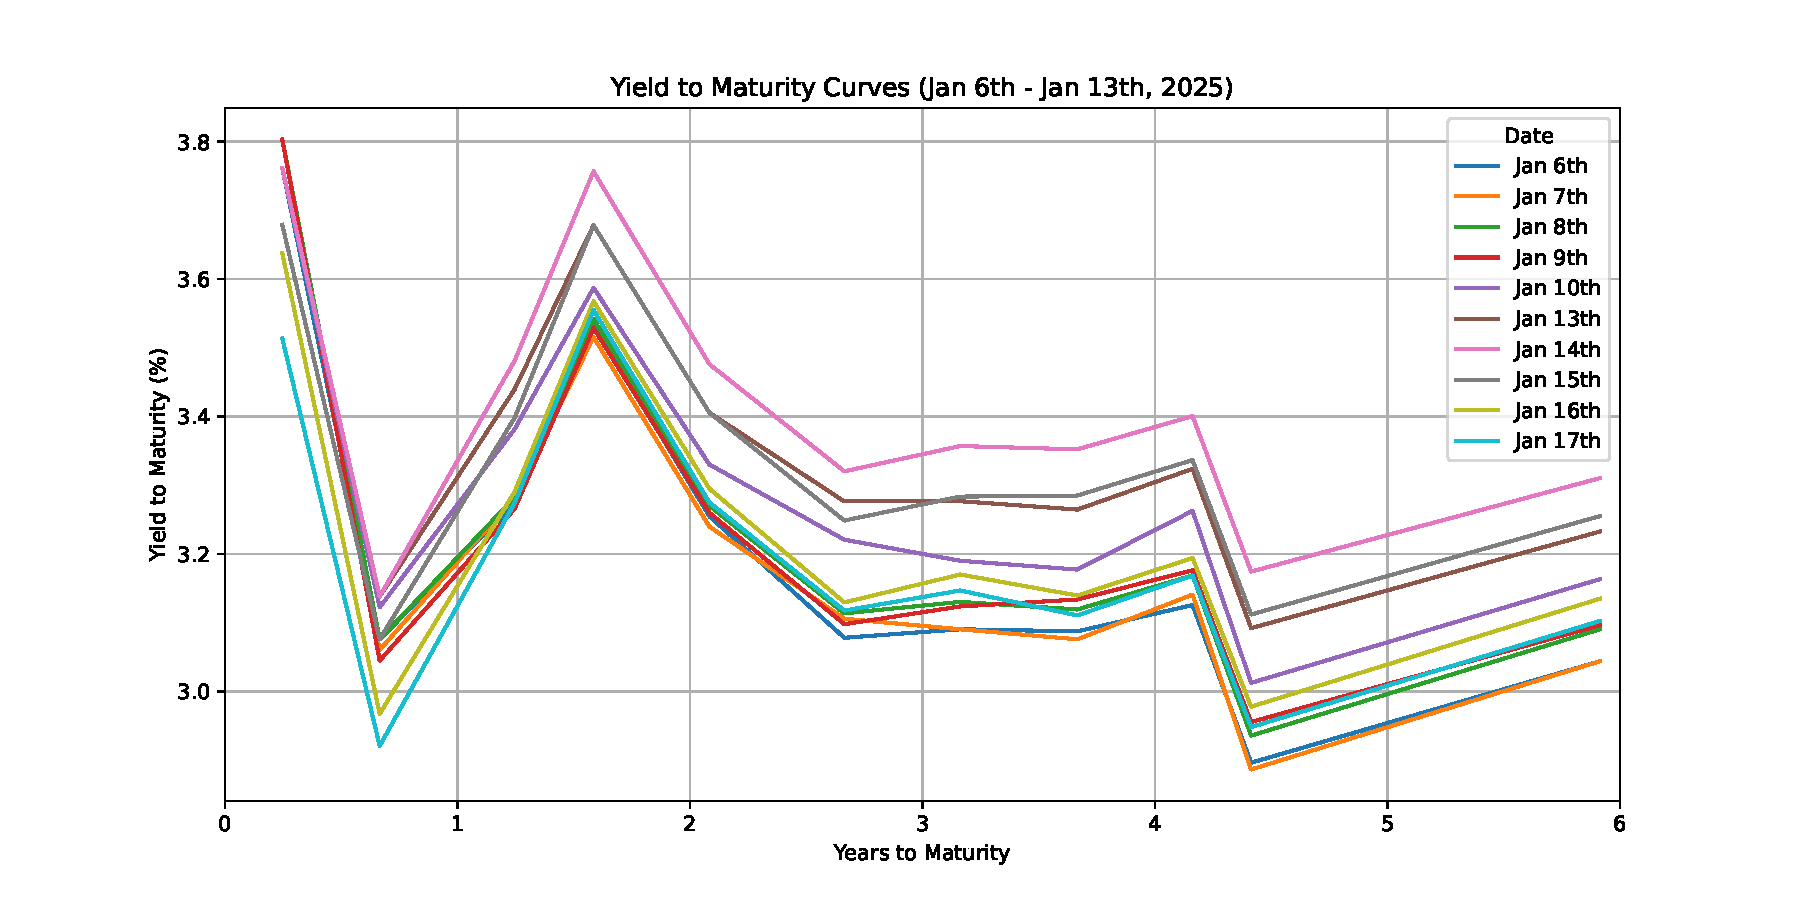
\includegraphics[width=0.8\textwidth]{ytm_curves.pdf} % Replace with your YTM plot file name
                \caption{Superimposed 5-Year Yield to Maturity (YTM) Curves for Each Trading Day}
                \label{fig:ytm_curves}
            \end{figure}

            Here we calculated the Yield to Maturity (YTM). Linear interpolation was employed to construct continuous curves from the discrete set of YTMs, to approximate the actual yield curve.

        \item \textbf{Spot Curve Derivation: Pseudo-code and Curves}

            To derive the spot curve, we employed the bootstrapping method, given by the pseudo-code below:

\begin{verbatim}
Function BootstrapSpotCurve(BondData, ValuationDate):
    SpotRates = {}
    Sort Bonds by Maturity (ascending)
    For each Bond:
        Given: Dirty Price (P), Coupon (C), Maturity Date
        MaturityYears = Years from ValuationDate to MaturityDate
        PVCoupons = 0
		For each Coupon Payment Time before Maturity:
            Discount coupon payment using bootstrapped SpotRate, add to PVCoupons
        ResidualPV = Dirty Price - PVCoupons
        SpotRate = ((Face Value + Last Coupon Payment) / 
        ResidualPV)$^{{(1 / MaturityYears)}}$ - 1
		Store SpotRate in SpotRates
	Return SpotRates
\end{verbatim}

            \item \textbf{Forward Curve Derivation: Pseudo-code and Curves}
            Here we derived the 1 year forward curves upto 4 years. The spot curve and forward curve plots are given below:
        \begin{enumerate}
            \begin{figure}[h!]
                \centering
                \begin{minipage}{0.48\textwidth} % Adjust width as needed, less than 0.5
                    \centering
                    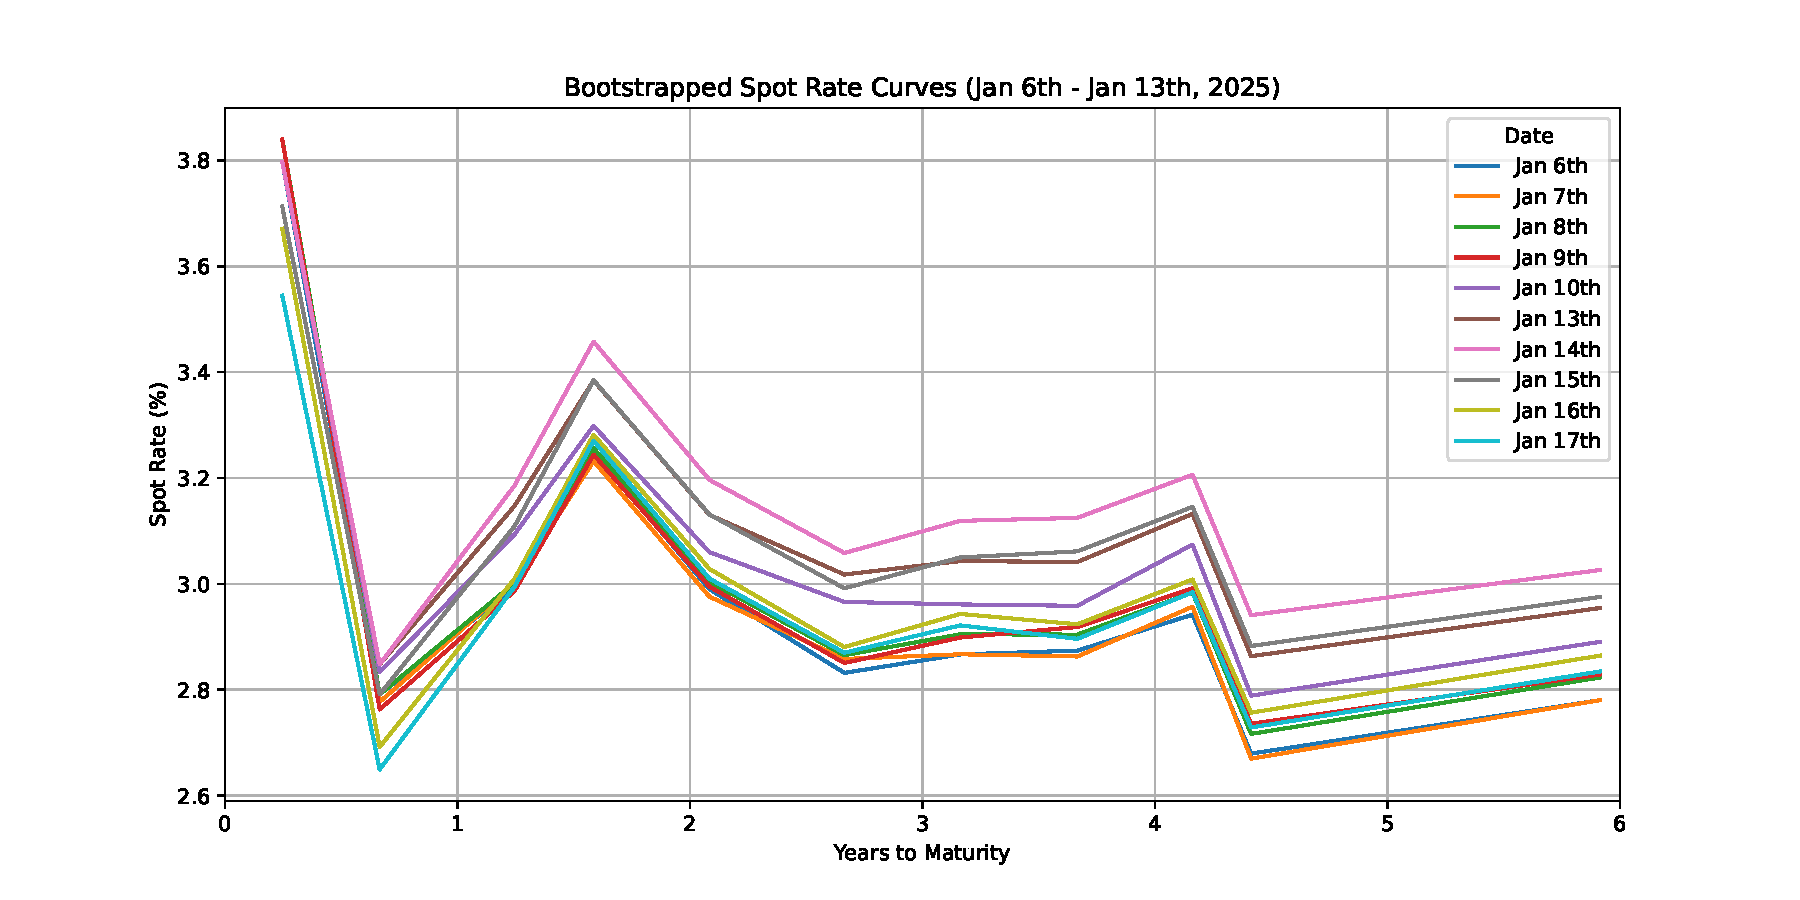
\includegraphics[width=\linewidth]{spot_curves.pdf} % Use \linewidth to fill minipage
                    \caption*{(a) Superimposed 5-Year Spot Rate Curves} % Sub-caption (a)
                    \label{fig:spot_curves}
                \end{minipage}
                \hfill % Horizontal space between minipages
                \begin{minipage}{0.48\textwidth} % Adjust width as needed, less than 0.5
                    \centering
                    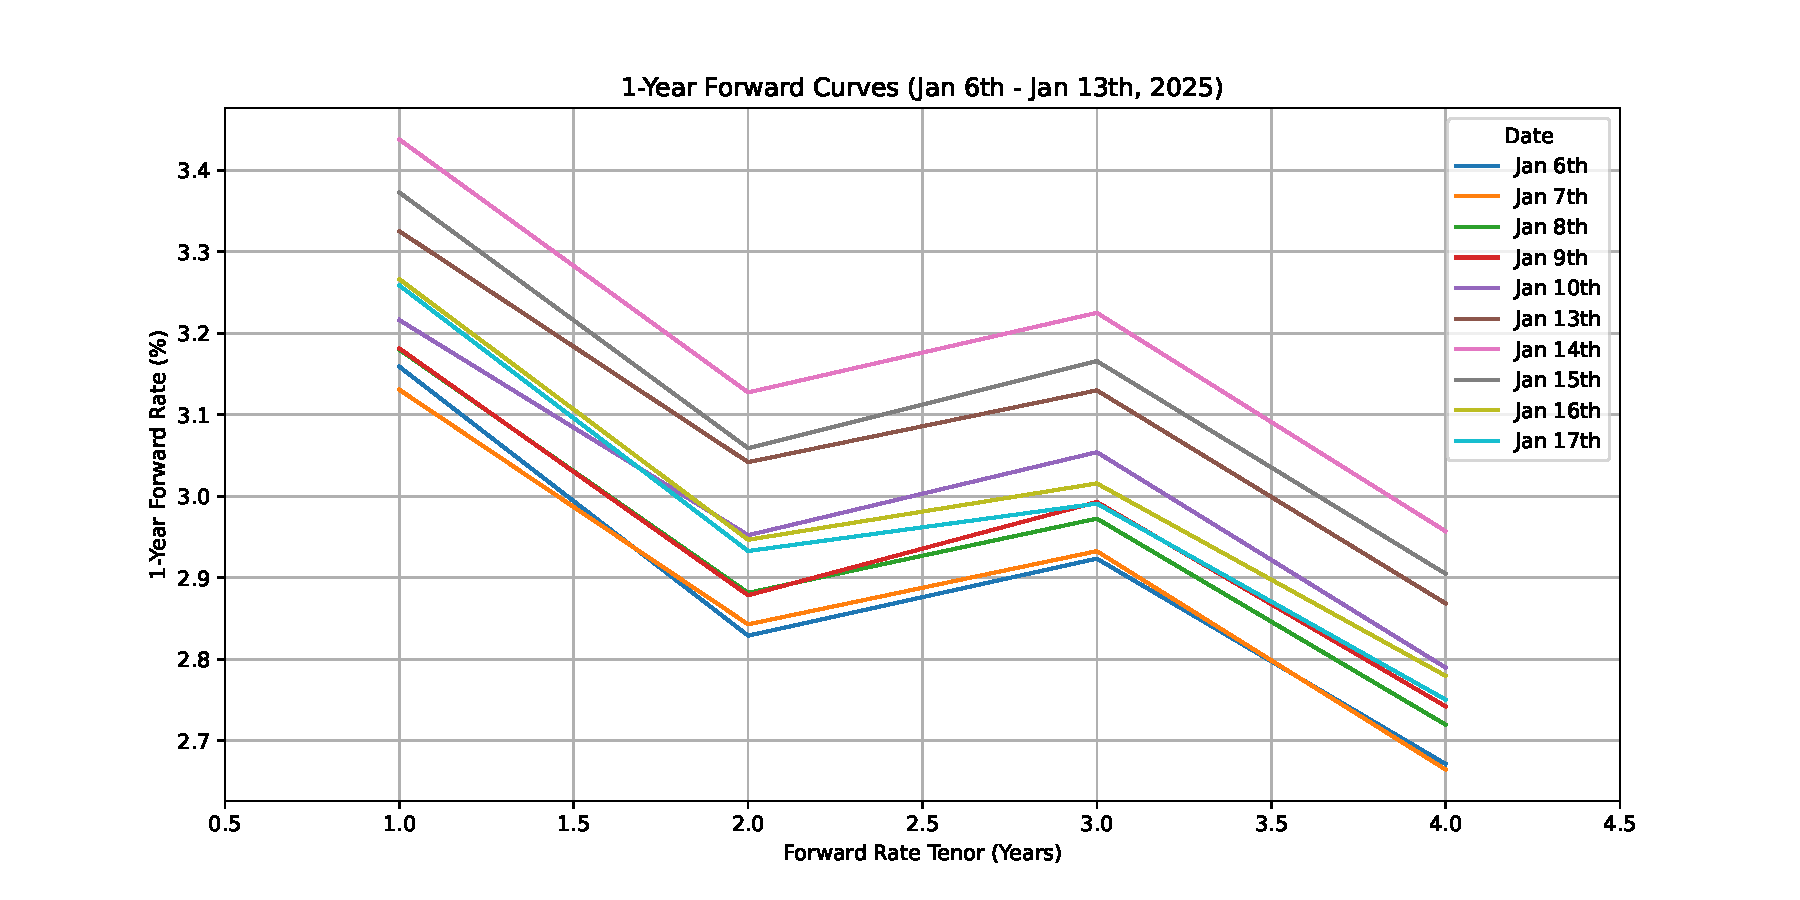
\includegraphics[width=\linewidth]{forward_curves.pdf} % Use \linewidth to fill minipage
                    \caption*{(b) Superimposed 1-Year Forward Curves} % Sub-caption (b)
                    \label{fig:forward_curves}
                \end{minipage}
                \caption{Spot Rate Curves and Forward Rate Curves for Each Trading Day} % Main caption for the combined figure
                \label{fig:spot_and_forward_curves} 
            \end{figure}
            
\begin{verbatim}
Function DeriveForwardCurve(SpotCurve):
    ForwardRates = {}
    ForwardTerms = [1, 2, 3, 4]
    StartTerm = 1.0
	For each ForwardTenor in ForwardTerms:
        EndTerm = StartTerm + ForwardTenor
        SpotRateStart = Interpolate SpotCurve at StartTerm
        SpotRateEnd = Interpolate SpotCurve at EndTerm
		ForwardRate =  (((1 + SpotRateEnd / 2)$^{{(2 * EndTerm)}}$) 		/
        ((1 + SpotRateStart / 2)^{{(2 * StartTerm)}}))$^{{(1 / 
        (2 * ForwardTenor))}}$ - 1

        Store ForwardRate in ForwardRates
    Return ForwardRates
\end{verbatim}
	\end{enumerate}
	\end{enumerate}

    \item \textbf{Covariance Matrices of Yield and Forward Rate Log-Returns}

        To analyze the co-movement and dynamics of the yield curve and forward rates, we calculated covariance matrices for the time series of daily log-returns. Prior to covariance matrix calculation, the log-returns were standardized (mean-centered and divided by standard deviation) to ensure that variables with different scales do not disproportionately influence the decomposition results.

\begin{table}[h!]
    \centering
    \begin{minipage}{0.48\textwidth}
        \centering
        \caption{Covariance Matrix of YTM Log Returns (Standardized)}
        \label{tab:covariance_ytm}
        \resizebox{\linewidth}{!}{% Resize table to fit within minipage width
        \[
        \begin{bmatrix}
            1.0000 & 0.7754 & 0.6754 & 0.7294 & 0.6399 \\
            0.7754 & 1.0000 & 0.9731 & 0.9695 & 0.9612 \\
            0.6754 & 0.9731 & 1.0000 & 0.9796 & 0.9778 \\
            0.7294 & 0.9695 & 0.9796 & 1.0000 & 0.9857 \\
            0.6399 & 0.9612 & 0.9778 & 0.9857 & 1.0000
        \end{bmatrix}
        \]
        }
    \end{minipage}
    \hfill
    \begin{minipage}{0.48\textwidth}
        \centering
        \caption{Covariance Matrix of Forward Rate Log Returns (Standardized)}
        \label{tab:covariance_forward}
        \resizebox{\linewidth}{!}{% Resize table to fit within minipage width
        \[
        \begin{bmatrix}
            1.0000 & 0.9711 & 0.9346 & 0.9643 \\
            0.9711 & 1.0000 & 0.9581 & 0.9681 \\
            0.9346 & 0.9581 & 1.0000 & 0.9855 \\
            0.9643 & 0.9681 & 0.9855 & 1.0000
        \end{bmatrix}
        \]
        }
    \end{minipage}
\end{table}

\item \textbf{Eigenvalues and Eigenvectors}

   	  The eigenvalue and eigenvector decomposition revealed the following:

    \textbf{For Yield to Maturity (YTM) Log-Returns:}
    \begin{itemize}
        \item \textbf{Eigenvalues:} $\lambda = [4.49, 0.45, 0.0034, 0.0320, 0.0178]$
        \item \textbf{Eigenvectors:}
        $V = \{ \mathbf{v_1} = [-0.47, -0.47, -0.46, -0.47, -0.46], \mathbf{v_2} = [0.90, -0.02, -0.25, -0.14, -0.32], \mathbf{v_3} = [0.18, -0.35, 0.27, -0.65, 0.60], \mathbf{v_4} = [0.10, -0.64, -0.37, 0.56, 0.37], \mathbf{v_5} = [-0.06, 0.50, -0.72, -0.18, 0.44] \}$
        The first eigenvalue being the largest means that it explains a majority of the variance in YTM log-returns, and the first eigenvector being approximately a vector of 1's indicates a level shift of the yield curve over time.  
    \end{itemize}

   \textbf{For Forward Rate Log-Returns:}
    \begin{itemize}
        \item \textbf{Eigenvalues:} $\lambda = [3.89, 0.073, 0.028, 0.0081]$
        \item \textbf{Eigenvectors:} 
        $V = \{ \mathbf{v_1} = [-0.49, -0.50, -0.49, -0.50], \mathbf{v_2} = [-0.65, -0.28, 0.65, 0.27], \mathbf{v_3} = [0.46, -0.80, -0.04, 0.38], \mathbf{v_4} = [-0.34, 0.17, -0.57, 0.73] \}$
        The first eigenvalue being the largest means that it explains a majority of the variance in forward rate log-returns, and the first eigenvector being approximately a vector of 1's indicates a level shift of the forward curve over time.  
    \end{itemize}

\end{enumerate}

\section*{References and GitHub Link to Code}

Github link: https://github.com/1raghav-bhatia/MathFinanceA1.git

\end{document}